% \documentclass[a4paper,landscape]{article}

\documentclass{standalone}

\usepackage[svgnames]{xcolor}
\usepackage{tikz}
\usetikzlibrary{calc}
\usetikzlibrary{decorations.markings}
\usetikzlibrary{shapes.geometric}


\pgfdeclarelayer{edgelayer}
\pgfdeclarelayer{nodelayer}
\pgfsetlayers{edgelayer,nodelayer,main}

\tikzstyle{none}=[inner sep=0pt]


%---------------------------------------------------
% Node styles
%---------------------------------------------------
\tikzstyle{ouput_layer_unit}=[fill={rgb,255: red,70; green,129; blue,255}, draw={rgb,255: red,8; green,0; blue,249}, shape=circle]

\tikzstyle{hidden_layer_unit}=[fill={rgb,255: red,147; green,255; blue,255}, draw={rgb,255: red,58; green,123; blue,180}, shape=circle]

\tikzstyle{empty_slot}=[fill=white, draw=black, shape=circle]

%\tikzstyle{mean}=[fill={rgb,255: red,247; green,255; blue,92}, draw={rgb,255: red,255; green,225; blue,70}, shape=circle]

%\tikzstyle{variance}=[fill={rgb,255: red,255; green,200; blue,112}, draw={rgb,255: red,188; green,109; blue,45}, shape=circle]

%\tikzstyle{latent_space}=[fill={rgb,255: red,75; green,193; blue,56}, draw={rgb,255: red,52; green,117; blue,49}, shape=circle]

\tikzstyle{parameter_vector_unit}=[fill={rgb,255: red,255; green,0; blue,4}, draw={rgb,255: red,107; green,0; blue,1}, shape=circle]

\tikzstyle{myText}=[fill=white, draw=white, shape=rectangle]

\tikzstyle{ellipsis}=[fill=black, draw=black, shape=circle]

\tikzstyle{rectangle}=[fill={rgb,255: red,98; green,255; blue,161}, draw=black, shape=rectangle]

%---------------------------------------------------
% Edge styles
%---------------------------------------------------
\tikzstyle{section_marker}=[{|-|}]
\tikzstyle{main_connector}=[-, draw={rgb,255: red,184; green,184; blue,184}]
\tikzstyle{secondary_concetor}=[-, draw={rgb,255: red,176; green,204; blue,229}, dashed]


\begin{document}

\pagestyle{empty}

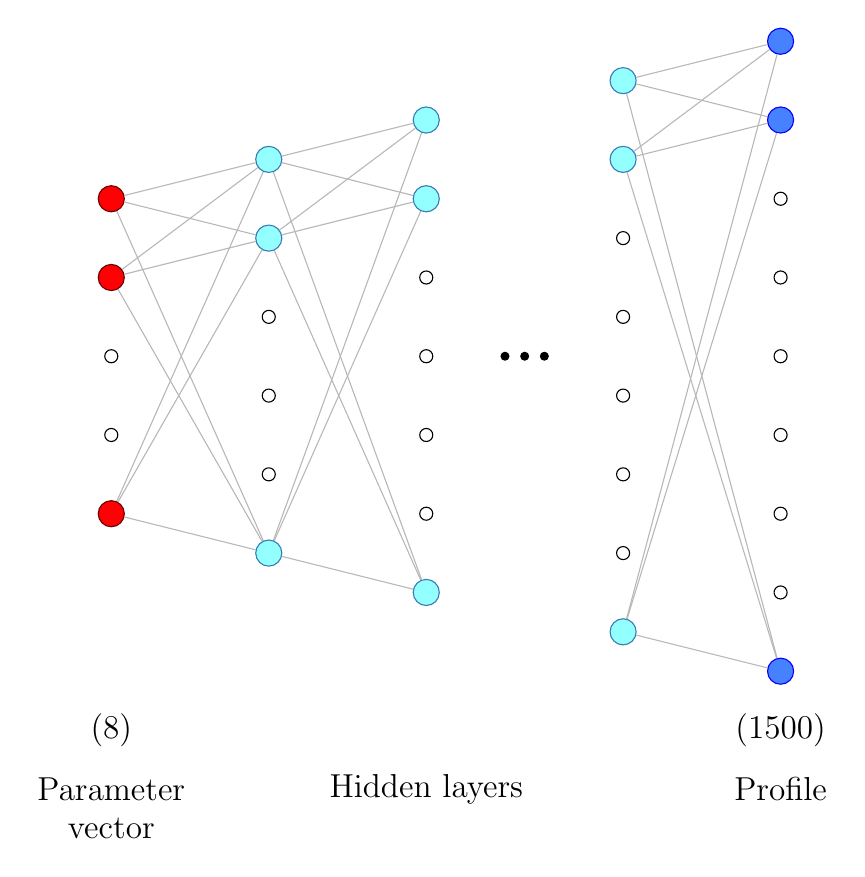
\begin{tikzpicture}
    \begin{pgfonlayer}{nodelayer}
        % input layer
        \node [style={parameter_vector_unit}] (0) at (0, 0) {};
        \node [style={parameter_vector_unit}] (3) at (0, 3) {};
        \node [style={parameter_vector_unit}] (4) at (0, 4) {};
        \node [style={empty_slot}, scale=0.5] (5) at (0, 2) {};
        \node [style={empty_slot}, scale=0.5] (6) at (0, 1) {};

        % first hidden layer
        \node [style={hidden_layer_unit}] (7) at (2, 4.5) {};
        \node [style={hidden_layer_unit}] (8) at (2, 3.5) {};
        \node [style={hidden_layer_unit}] (9) at (2, -0.5) {};
        \node [style={empty_slot}, scale=0.5] (11) at (2, 2.5) {};
        \node [style={empty_slot}, scale=0.5] (12) at (2, 1.5) {};
        \node [style={empty_slot}, scale=0.5] (13) at (2, 0.5) {};
        
        % second hidden layer
        \node [style={hidden_layer_unit}] (17) at (4, 5) {};
        \node [style={hidden_layer_unit}] (18) at (4, 4) {};
        \node [style={hidden_layer_unit}] (19) at (4, -1) {};
        \node [style={empty_slot}, scale=0.5] (21) at (4, 3) {};
        \node [style={empty_slot}, scale=0.5] (22) at (4, 2) {};
        \node [style={empty_slot}, scale=0.5] (23) at (4, 1) {};
        \node [style={empty_slot}, scale=0.5] (24) at (4, 0) {};

        % ellipsis    
        \node [style=ellipsis, scale=0.3] (34) at (5.0, 2) {};
        \node [style=ellipsis, scale=0.3] (35) at (5.25, 2) {};
        \node [style=ellipsis, scale=0.3] (36) at (5.5, 2) {};
        
        % final hidden layer
        \node [style={hidden_layer_unit}] (37) at (6.5, 4.5) {};
        \node [style={hidden_layer_unit}] (38) at (6.5, 5.5) {};
        \node [style={hidden_layer_unit}] (39) at (6.5, -1.5) {};
        \node [style={empty_slot}, scale=0.5] (29) at (6.5, 3.5) {};
        \node [style={empty_slot}, scale=0.5] (30) at (6.5, 2.5) {};
        \node [style={empty_slot}, scale=0.5] (31) at (6.5, 1.5) {};
        \node [style={empty_slot}, scale=0.5] (32) at (6.5, 0.5) {};
        \node [style={empty_slot}, scale=0.5] (33) at (6.5, -0.5) {};

        % output layer
        \node [style=ouput_layer_unit] (40) at (8.5, 6) {};
        \node [style=ouput_layer_unit] (41) at (8.5, 5) {};
        \node [style=ouput_layer_unit] (42) at (8.5, -2) {};
        \node [style={empty_slot}, scale=0.5] (43) at (8.5, 4) {};
        \node [style={empty_slot}, scale=0.5] (44) at (8.5, 3) {};
        \node [style={empty_slot}, scale=0.5] (45) at (8.5, 2) {};
        \node [style={empty_slot}, scale=0.5] (46) at (8.5, 1) {};
        \node [style={empty_slot}, scale=0.5] (47) at (8.5, 0) {};
        \node [style={empty_slot}, scale=0.5] (48) at (8.5, -1) {};
        
        
        % description at the bottom 
        \node [style=myText] (50) at (0, -2.75) {\large (8)};
        \node [style=myText] (51) at (0, -3.5) {\large Parameter};
        \node [style=myText] (52) at (0, -4.0) {\large vector};

        \node [style=myText] (60) at (8.5, -2.75) {\large (1500)};
        \node [style=myText] (61) at (8.5, -3.5) {\large Profile};
        
        \node [style=myText] (51) at (4, -3.5) {\large Hidden layers};
        
        % epmty nodes for docking line at the bottom 
        \node [style=none] (100) at (1.75,  -2.75) {};
        \node [style=none] (101) at (6.25,  -2.75) {};
        
    \end{pgfonlayer}
    \begin{pgfonlayer}{edgelayer}
        \draw [style={main_connector}] (4) to (7);
        \draw [style={main_connector}] (4) to (8);
        \draw [style={main_connector}] (4) to (9);
        \draw [style={main_connector}] (3) to (7);
        \draw [style={main_connector}] (3) to (8);
        \draw [style={main_connector}] (3) to (9);
        \draw [style={main_connector}] (0) to (9);
        \draw [style={main_connector}] (0) to (8);
        \draw [style={main_connector}] (0) to (7);
        \draw [style={main_connector}] (7) to (17);
        \draw [style={main_connector}] (7) to (18);
        \draw [style={main_connector}] (8) to (18);
        \draw [style={main_connector}] (8) to (17);
        \draw [style={main_connector}] (7) to (19);
        \draw [style={main_connector}] (8) to (19);
        \draw [style={main_connector}] (19) to (9);
        \draw [style={main_connector}] (9) to (18);
        \draw [style={main_connector}] (9) to (17);
        \draw [style={main_connector}] (38) to (40);
        \draw [style={main_connector}] (38) to (41);
        \draw [style={main_connector}] (37) to (40);
        \draw [style={main_connector}] (38) to (42);
        \draw [style={main_connector}] (42) to (39);
        \draw [style={main_connector}] (39) to (41);
        \draw [style={main_connector}] (40) to (39);
        \draw [style={main_connector}] (37) to (41);
        \draw [style={main_connector}] (37) to (42);
        
        
        %\draw [style={section_marker}] (100) to (101);
        
    \end{pgfonlayer}
\end{tikzpicture}



\end{document}
